%  !TeX  root  =  user_guide.tex

\section{Plugin GPS}\label{label_plugingps}

% when the revision of a section has been finalized,
% comment out the following line:
% \updatedisclaimer

\subsection{Cosa è il GPS?}\label{whatsgps}

GPS sta per Global Positioning System ed indica un sistema satellitare che permette a chiunque possegga 
un ricevitore GPS di trovare la propria posizione ovunque nel mondo.
Viene usato come ausilio nella navigazione, ad esempio in aereo, in barca o anche per semplici escursioni.
Il ricevitore GPS usa i segnali provenienti dai satelliti per calcolare la propria latitudine, longitudine 
e (talvolta) elevazione.
La maggior parte dei ricevitori ha anche la capacità di archiviare posizioni (note come \emph{waypoint}), 
sequenze di posizioni che costituiscono una rotta o \emph{route} pianificata e una traccia o \emph{track} 
dei propri movimenti nel tempo.
Waypoint, route e track sono i tre elementi base dei dati GPS.
QGIS mostra i waypoint in layer di punti, mentre route e track vengono mostrate in layer di linee.

\subsection{Caricare i dati GPS da un file}\label{label_loadgps}

Ci sono dozzine di diversi formati di file per archiviare dati GPS. Il formato usato da QGIS si chiama GPX 
(GPS eXchange format, formato di scambio GPS), un formato standard di interscambio che può contenere 
qualunque numero di waypoint, route e track nello stesso file.

Per caricare un file GPX bisogna prima caricare il plugin
\mainmenuopt{Plugins} \arrow \dropmenuopttwo{mActionShowPluginManager}{Gestione plugins...} \arrow 
\checkbox{Strumenti GPS}. Caricato il plugin, un tasto indicante un piccolo dispositivo manuale GPS compare 
nella barra degli strumenti gestione layer. Un file GPX di esempio è disponibile nel dataset:
\filename{/qgis\_sample\_data/gps/national\_monuments.gpx}. Si veda la Sezione~\ref{label_sampledata} 
per avere maggiori informazioni sui dati di esempio.

\begin{enumerate}
\item Cliccare su \toolbtntwo{gps_importer}{Strumenti GPS} e selezionare la scheda \tab{Carica file GPX}.
\item \button{Sfoglia} la cartella \filename{qgis\_sample\_data/gps/},
selezionare il file GPX \filename{national\_monuments.gpx} e cliccare su \button{Apri}.
\item Selezionare con le caselle di controllo i tipi di dati che si desidera caricare dal file GPX.
\item Cliccare su \button{OK} per visualizzare i dati in QGIS: il file \filename{national\_monuments.gpx} 
contiene soltanto waypoint.
\end{enumerate}

\begin{figure}[ht]
   \centering
   \includegraphics[clip=true, width=12cm]{loadgpx}
   \caption{Finestra di dialogo \emph{Strumenti GPS} \nixcaption}\label{gpxloader}
\end{figure}

\subsection{GPSBabel}

Dato che QGIS usa file in formato GPX, è necessario un sistema per convertire altri formati di file GPS in GPX.
Questo può essere fatto per molti formati usando il programma gratuito GPSBabel, che è disponibile alla
pagine web \url{http://www.gpsbabel.org}.
GPSBabel può anche trasferire i dati GPS tra il computer e il dispositivo GPS: QGIS usa GPSBabel per le stesse 
operazioni, per cui si raccomanda di installare il programma. Tuttavia, se si vuole solamente caricare dati GPS 
da file GPX, l'installazione non è necessaria.
È noto che la versione 1.2.3 di GPSBabel funziona con QGIS, ma non ci dovrebbero essere problemi anche con 
versioni successive.

\subsection{Importare dati GPS}

Per importare dati GPS da un file che non è in formato GPX, si può usare lo strumento \tab{Importa un altro file} 
nella finestra di dialogo Strumenti GPS.
Selezionare il file che si vuole importare, quali tipi di dati si vogliono importare da esso, dove deve essere 
archiviato il file convertito GPX e quale deve essere il nome del nuovo layer. Non tutti i formati dati GPS supportano 
i tipi di dati del plugin: per alcuni formati sarà possibile selezionare solo alcuni tipi.

\subsection{Scaricare dati GPS da un dispositivo}

QGIS può usare GPSBabel per scaricare i dati da un dispositivo GPS direttamente in layer vettoriali.
Per questa operazione si usa la scheda \tab{Scarica dal GPS} (Figura \ref{figure_download}), 
dove si seleziona il tipo di dispositivo GPS, la porta di comunicazione alla quale è connesso, 
i tipi di dati che si vogliono scaricare, il nome del file GPX dove i dati devono essere archiviati e 
il nome del nuovo layer.

\begin{figure}[ht]
   \centering
   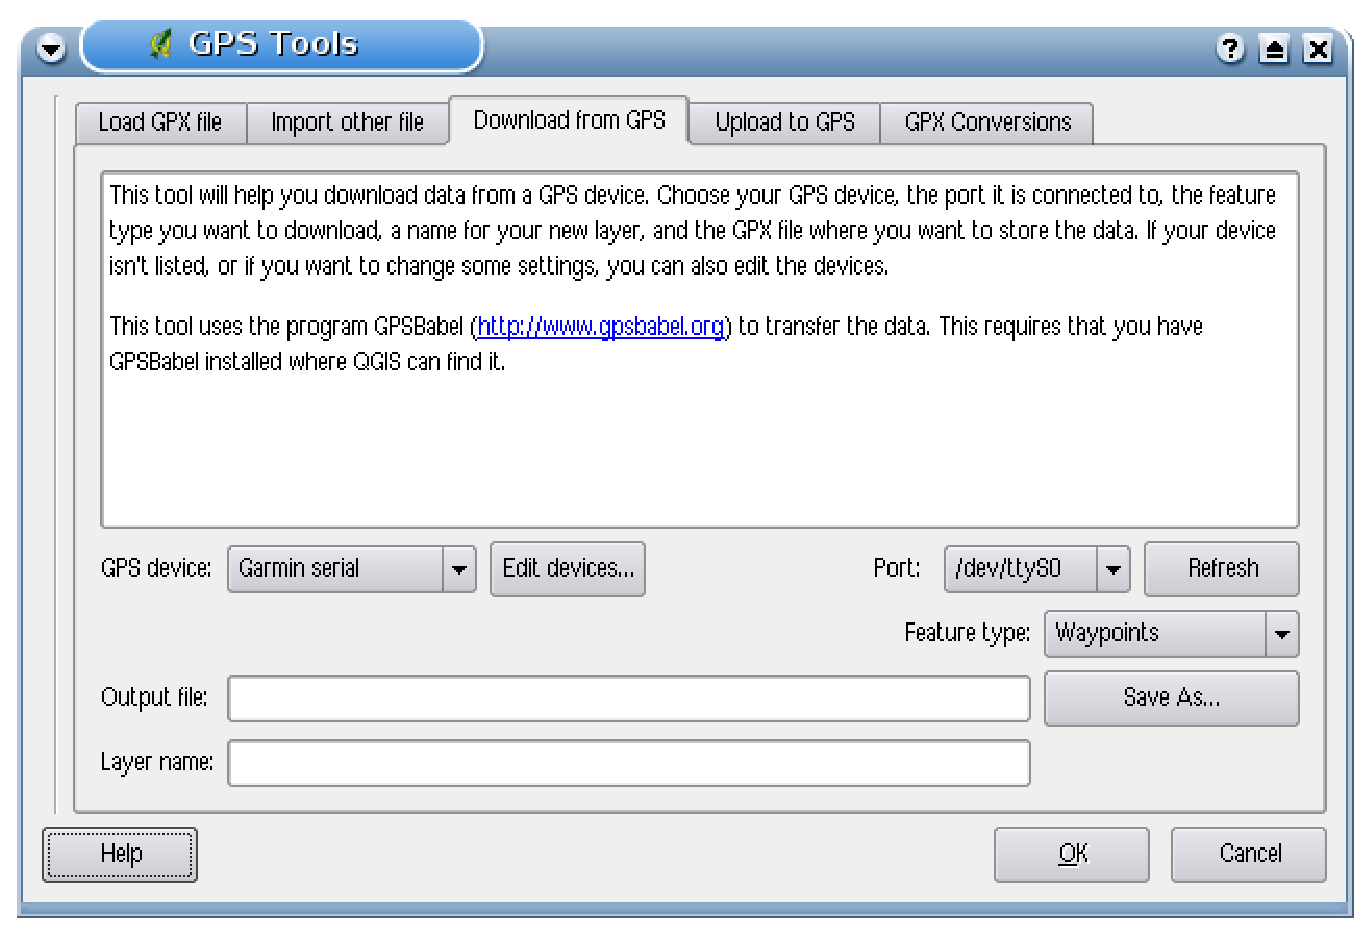
\includegraphics[clip=true, width=12cm]{download}
   \caption{La scheda Scarica dal GPS \nixcaption}\label{figure_download}
\end{figure}

Il tipo di dispositivo che si seleziona nel menu dispositivi GPS determina il modo con cui GPSBabel 
cerca di comunicare con il dispositivo in questione. Se nessuno di questi tipi funziona con il 
dispositivo che si ha, si può creare un nuovo tipo (Sezione \ref{sec:Defining-new-device}).

La porta può essere un nome di file o un qualche altro nome che il sistema operativo usa per riferirsi 
alla porta fisica del computer cui è connesso il dispositivo GPS (potrebbe semplicemente essere usb): 
\nix in Linux è qualcosa come /dev/ttyS0 or /dev/ttyS1 e in \win Windows è COM1 o COM2.

Cliccando su \button{OK} i dati vengono scaricati dal dispositivo ed appaiono come layer in QGIS.

\subsection{Caricare dati GPS su un dispositivo}

Si può anche caricare dati direttamente da un layer vettoriale di QGIS su un dispositivo GPS, 
usando la scheda \tab{Carica sul GPS}. Il layer deve essere un file GPX: si seleziona il layer che si 
vuole caricare, il tipo di dispositivo GPS e la porta cui è connesso.
Bisogna specificare un nuovo tipo di dispositivo se quello che si sta usando non è nella lista delle 
periferiche GPS.

Questo strumento è molto utile in combinazione alle capacità di modifica vettoriale di QGIS.
Si può lavorare su una mappa, creare alcuni waypoint e route e poi caricarli ed utilizzarli nel proprio 
dispositivo GPS.

\subsection{Definire un nuovo dispositivo}\label{sec:Defining-new-device}

Ci sono molti tipi di dispositivi GPS. Gli sviluppatori di QGIS non possono testarli tutti: se si 
possiede un dispositivo che non funziona con nessuno dei tipi elencati nelle schede 
\tab{Scarica dal GPS} e \tab{Carica sul GPS}, si può definire il proprio tipo di dispositivo usando 
l'Editor delle periferiche GPS, che si apre cliccando su \button{Modifica periferiche}.

Per definire un nuovo dispositivo, basta cliccare su \button{Nuovo}, scegliere un nome, un comando per scaricare 
(download) ed uno per caricare (upload) i dati ed infine cliccare su \button{Aggiorna}.
Il nuovo dispositivo verrà elencato nel menu dei dispositivi.
Il comando di download è il comando usato per scaricare i dati dal dispositivo GPS in un file GPX.
Questo probabilmente sarà un comando di GPSBabel, ma si può usare qualunque altra linea di comando che 
possa creare un file GPX. 

QGIS sostituirà le parole chiave \usertext{\%type}, \usertext{\%in}, and \usertext{\%out}. \usertext{\%type} sarà 
sostituito da {}``\usertext{-w}'' se si stanno scaricando waypoint, {}``\usertext{-r}'' se si stanno scaricando route 
e {}``\usertext{-t}'' se si stanno scaricando track: queste sono opzioni della linea di comando che dicono a 
GPSBabel quali tipi di dati scaricare.

\usertext{\%in} sarà sostituito dal nome della porta scelta nella finestra di dialogo di download e 
\usertext{\%out} sarà sostituito dal nome scelto per il file GPX in cui saranno archiviati i dati scaricati.
Così, se si crea un dispositivo con il comando di download {}``\usertext{gpsbabel \%type -i garmin -o gpx \%in \%out}'' 
(questo è in realtà il comando di dowload per il tipo di dispositivo predefinto \selectstring{GPS device:}{Garmin serial}) 
e lo si usa poi per scaricare waypoints dalla porta {}``\usertext{/dev/ttyS0}'' al file {}``\usertext{output.gpx}'', 
QGIS sostituirà le parole chiave ed eseguirà il comando {}``\usertext{gpsbabel -w -i garmin -o gpx /dev/ttyS0 output.gpx}''.

Il comando di upload è il comando che si usa per caricare dati sul disposiyivo GPS.
Si usano le stesse parole chiave, ma \usertext{\%in} è sostituito con il nome del file GPX per il layer che si sta caricando 
e \usertext{\%out} è sostituito dal nome della porta.

Per ulteriori informazioni su GPSBabel: \url{http://www.gpsbabel.org}

\FloatBarrier